% Options for packages loaded elsewhere
\PassOptionsToPackage{unicode}{hyperref}
\PassOptionsToPackage{hyphens}{url}
%
\documentclass[
  12pt,
]{article}
\usepackage{amsmath,amssymb}
\usepackage{lmodern}
\usepackage{ifxetex,ifluatex}
\ifnum 0\ifxetex 1\fi\ifluatex 1\fi=0 % if pdftex
  \usepackage[T1]{fontenc}
  \usepackage[utf8]{inputenc}
  \usepackage{textcomp} % provide euro and other symbols
\else % if luatex or xetex
  \usepackage{unicode-math}
  \defaultfontfeatures{Scale=MatchLowercase}
  \defaultfontfeatures[\rmfamily]{Ligatures=TeX,Scale=1}
\fi
% Use upquote if available, for straight quotes in verbatim environments
\IfFileExists{upquote.sty}{\usepackage{upquote}}{}
\IfFileExists{microtype.sty}{% use microtype if available
  \usepackage[]{microtype}
  \UseMicrotypeSet[protrusion]{basicmath} % disable protrusion for tt fonts
}{}
\makeatletter
\@ifundefined{KOMAClassName}{% if non-KOMA class
  \IfFileExists{parskip.sty}{%
    \usepackage{parskip}
  }{% else
    \setlength{\parindent}{0pt}
    \setlength{\parskip}{6pt plus 2pt minus 1pt}}
}{% if KOMA class
  \KOMAoptions{parskip=half}}
\makeatother
\usepackage{xcolor}
\IfFileExists{xurl.sty}{\usepackage{xurl}}{} % add URL line breaks if available
\IfFileExists{bookmark.sty}{\usepackage{bookmark}}{\usepackage{hyperref}}
\hypersetup{
  pdftitle={Stand Up Fight Back},
  pdfauthor={Kevin Morris; Kelsey Shoub},
  hidelinks,
  pdfcreator={LaTeX via pandoc}}
\urlstyle{same} % disable monospaced font for URLs
\usepackage[margin=1in]{geometry}
\usepackage{longtable,booktabs,array}
\usepackage{calc} % for calculating minipage widths
% Correct order of tables after \paragraph or \subparagraph
\usepackage{etoolbox}
\makeatletter
\patchcmd\longtable{\par}{\if@noskipsec\mbox{}\fi\par}{}{}
\makeatother
% Allow footnotes in longtable head/foot
\IfFileExists{footnotehyper.sty}{\usepackage{footnotehyper}}{\usepackage{footnote}}
\makesavenoteenv{longtable}
\usepackage{graphicx}
\makeatletter
\def\maxwidth{\ifdim\Gin@nat@width>\linewidth\linewidth\else\Gin@nat@width\fi}
\def\maxheight{\ifdim\Gin@nat@height>\textheight\textheight\else\Gin@nat@height\fi}
\makeatother
% Scale images if necessary, so that they will not overflow the page
% margins by default, and it is still possible to overwrite the defaults
% using explicit options in \includegraphics[width, height, ...]{}
\setkeys{Gin}{width=\maxwidth,height=\maxheight,keepaspectratio}
% Set default figure placement to htbp
\makeatletter
\def\fps@figure{htbp}
\makeatother
\setlength{\emergencystretch}{3em} % prevent overfull lines
\providecommand{\tightlist}{%
  \setlength{\itemsep}{0pt}\setlength{\parskip}{0pt}}
\setcounter{secnumdepth}{5}
\usepackage{rotating}
\usepackage{setspace}
\usepackage{booktabs}
\usepackage{longtable}
\usepackage{array}
\usepackage{multirow}
\usepackage{wrapfig}
\usepackage{float}
\usepackage{colortbl}
\usepackage{pdflscape}
\usepackage{tabu}
\usepackage{threeparttable}
\usepackage{threeparttablex}
\usepackage[normalem]{ulem}
\usepackage{makecell}
\usepackage{xcolor}
\ifluatex
  \usepackage{selnolig}  % disable illegal ligatures
\fi
\newlength{\cslhangindent}
\setlength{\cslhangindent}{1.5em}
\newlength{\csllabelwidth}
\setlength{\csllabelwidth}{3em}
\newenvironment{CSLReferences}[2] % #1 hanging-ident, #2 entry spacing
 {% don't indent paragraphs
  \setlength{\parindent}{0pt}
  % turn on hanging indent if param 1 is 1
  \ifodd #1 \everypar{\setlength{\hangindent}{\cslhangindent}}\ignorespaces\fi
  % set entry spacing
  \ifnum #2 > 0
  \setlength{\parskip}{#2\baselineskip}
  \fi
 }%
 {}
\usepackage{calc}
\newcommand{\CSLBlock}[1]{#1\hfill\break}
\newcommand{\CSLLeftMargin}[1]{\parbox[t]{\csllabelwidth}{#1}}
\newcommand{\CSLRightInline}[1]{\parbox[t]{\linewidth - \csllabelwidth}{#1}\break}
\newcommand{\CSLIndent}[1]{\hspace{\cslhangindent}#1}

\title{Stand Up Fight Back\thanks{Thanks.}}
\usepackage{etoolbox}
\makeatletter
\providecommand{\subtitle}[1]{% add subtitle to \maketitle
  \apptocmd{\@title}{\par {\large #1 \par}}{}{}
}
\makeatother
\subtitle{How Police Killings Can Mobilize Local Communities}
\author{Kevin Morris\footnote{Brennan Center for Justice, Researcher (\href{mailto:kevin.morris@nyu.edu}{\nolinkurl{kevin.morris@nyu.edu}})} \and Kelsey Shoub\footnote{University of South Carolina, Assistant Professor (\href{mailto:kshoub@mailbox.sc.edu}{\nolinkurl{kshoub@mailbox.sc.edu}})}}
\date{October 27, 2021}

\begin{document}
\maketitle
\begin{abstract}
TKTKTKTK
\end{abstract}

\pagenumbering{gobble}
\pagebreak
\doublespacing

\pagenumbering{arabic}

\hypertarget{data}{%
\section*{Data}\label{data}}
\addcontentsline{toc}{section}{Data}

\begin{itemize}
\item
  Combine the WaPo dataset (\url{https://www.washingtonpost.com/graphics/investigations/police-shootings-database/}) with the Mapping Police Violence data (\url{https://mappingpoliceviolence.org/}).
\item
  National (geocoded) voter files following each of the 2014, 2016, 2018, and 2020 elections from L2 Political. We use the voter file to calculate the number of ballots cast in each block group; we divide this number by 5-year CVAP estimates to construct turnout
\item
  Precinct-level shapefiles and results data from Mike McDonald (\url{https://dataverse.harvard.edu/dataverse/electionscience}). We've got 42 states as of Oct 4
\item
  Measure the distance between each block group / precinct and the closest police killing in the 2 months before and after each election
\end{itemize}

\hypertarget{empirical-setup}{%
\section*{Empirical Setup}\label{empirical-setup}}
\addcontentsline{toc}{section}{Empirical Setup}

We use a regression discontinuity in time to test whether block groups within a certain radius of a police killing immediately before an election turnout and vote at different rates than those with a killing immediately following the election.

Specifically, we retain block groups whose centroids are within 0.5 miles (in our primary model) of a killing before \emph{or} (but not \emph{and}) after the election. In other words, block groups who were close to a killing before and after the election are excluded.

Same deal with Biden's voteshare by precinct using the precinct data.

Regression discontinuity assumes that there's no difference between units on either side of the cutoff; no reason to think that violation is violated here. But, block groups close to a killing after the election do look a little different. Thus, we use entropy balancing to weight the block groups with a post-election killing so they look the same as the pre-election block groups.

Across the board, we're using the \texttt{rdrobust} package that implements an automated bandwidth selection procedure and allows for robust and biased-corrected estimates standard errors (\protect\hyperlink{ref-Calonico2014}{Calonico, Cattaneo, and Titiunik 2014}). This follows the advice of a working paper tearing apart like every RDD in \emph{APSR}, \emph{AJPS}, and \emph{JOP} from the past few years (\protect\hyperlink{ref-Stommes2021}{Stommes, Aronow, and Sävje 2021}).

\hypertarget{early-results}{%
\section*{Early Results}\label{early-results}}
\addcontentsline{toc}{section}{Early Results}

\begin{figure}[h]

{\centering 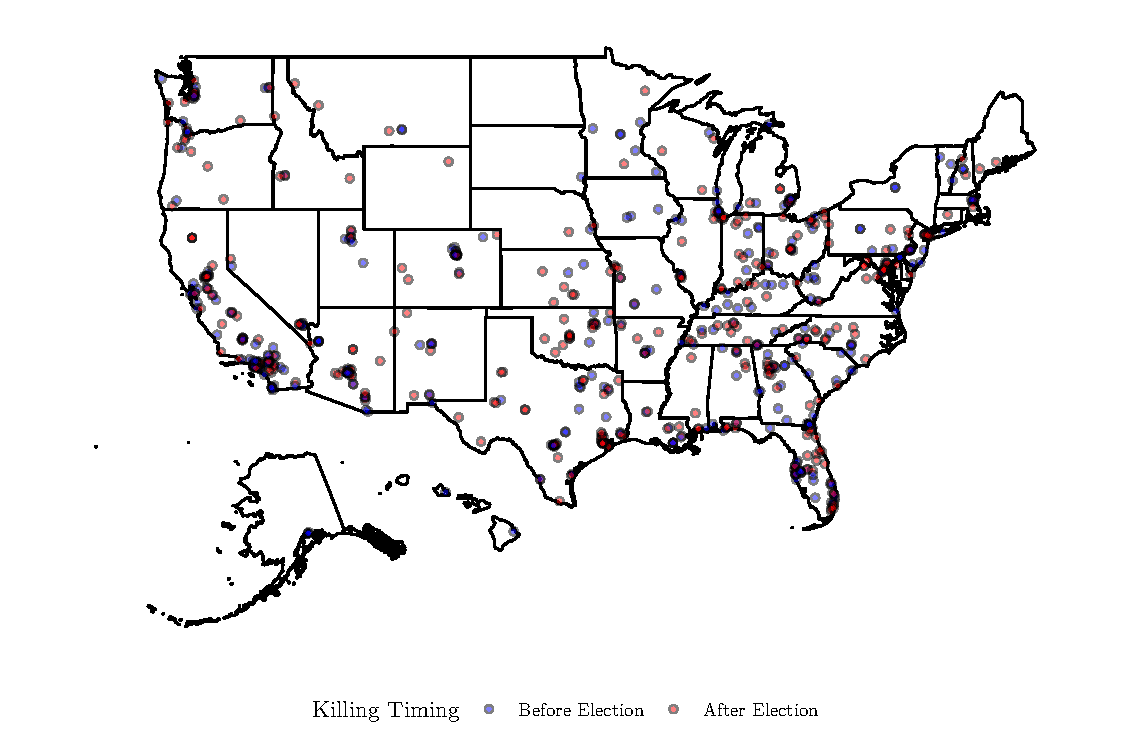
\includegraphics{shoot_to_files/figure-latex/map-chunk-1} 

}

\caption{\label{fig:map}Police Killing within 2 Months of Election, 2016 and 2020}\label{fig:map-chunk}
\end{figure}

\begin{singlespace}
\begin{table}[H]

\caption{\label{tab:balance-tab-full}\label{tab:full-bal} Demographics of Block Groups with Police Killings}
\centering
\begin{tabular}[t]{l>{\raggedright\arraybackslash}p{1in}>{\raggedright\arraybackslash}p{1in}>{\raggedright\arraybackslash}p{1in}>{\raggedright\arraybackslash}p{1in}}
\toprule
 & Not in Dataset & Treated & Unweighted Controls & Weighted Controls\\
\midrule
\addlinespace[0.3em]
\multicolumn{5}{l}{\textbf{2016}}\\
\hspace{1em}\% White & 63.3\% & 38.3\% & 31.7\% & 38.3\%\\
\hspace{1em}\% Black & 12.5\% & 20.9\% & 32.0\% & 20.9\%\\
\hspace{1em}\% Latino & 16.0\% & 29.1\% & 29.2\% & 29.1\%\\
\hspace{1em}\% Asian & 4.7\% & 8.2\% & 4.2\% & 8.2\%\\
\hspace{1em}Median Age & 40.6 & 36.4 & 34.6 & 36.4\\
\hspace{1em}Median Income & \$69,119 & \$51,999 & \$43,402 & \$51,999\\
\hspace{1em}Population Density & 6,130 & 16,112 & 19,164 & 16,112\\
\hspace{1em}Previous Turnout & 35.9\% & 28.5\% & 26.6\% & 28.5\%\\
\addlinespace[0.3em]
\multicolumn{5}{l}{\textbf{2020}}\\
\hspace{1em}\% White & 63.0\% & 38.1\% & 31.4\% & 38.1\%\\
\hspace{1em}\% Black & 12.6\% & 16.6\% & 29.9\% & 16.6\%\\
\hspace{1em}\% Latino & 16.2\% & 37.5\% & 28.7\% & 37.5\%\\
\hspace{1em}\% Asian & 4.7\% & 4.4\% & 6.4\% & 4.4\%\\
\hspace{1em}Median Age & 40.6 & 36.3 & 36.4 & 36.3\\
\hspace{1em}Median Income & \$69,365 & \$54,935 & \$55,469 & \$54,935\\
\hspace{1em}Population Density & 6,208 & 24,550 & 26,470 & 24,550\\
\hspace{1em}Previous Turnout & 49.6\% & 44.7\% & 40.2\% & 44.7\%\\
\bottomrule
\end{tabular}
\end{table}
\end{singlespace}

Clearly, police killings happen A) in less white, more Black areas, B) in lower-income and denser areas, and C) places with lower turnout in 2014 and 2018.

Primary RD plot using a 0.5-mile radius around the killings. This uses entropy balancing \emph{and} covariates.

\begin{figure}[H]

{\centering 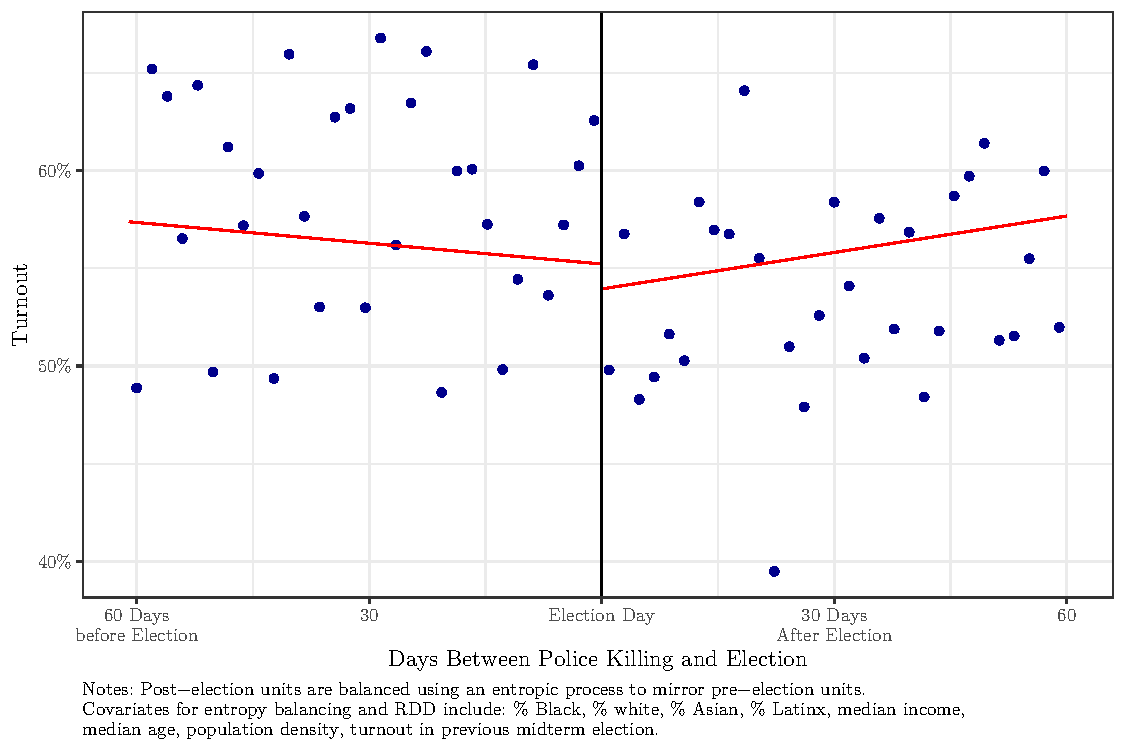
\includegraphics{shoot_to_files/figure-latex/rd1-chunk-1} 

}

\caption{\label{fig:map}RDD Plot, EB + Covariates, 2016 and 2020}\label{fig:rd1-chunk}
\end{figure}

Now no entropy balancing, only covariates:

\begin{figure}[H]

{\centering 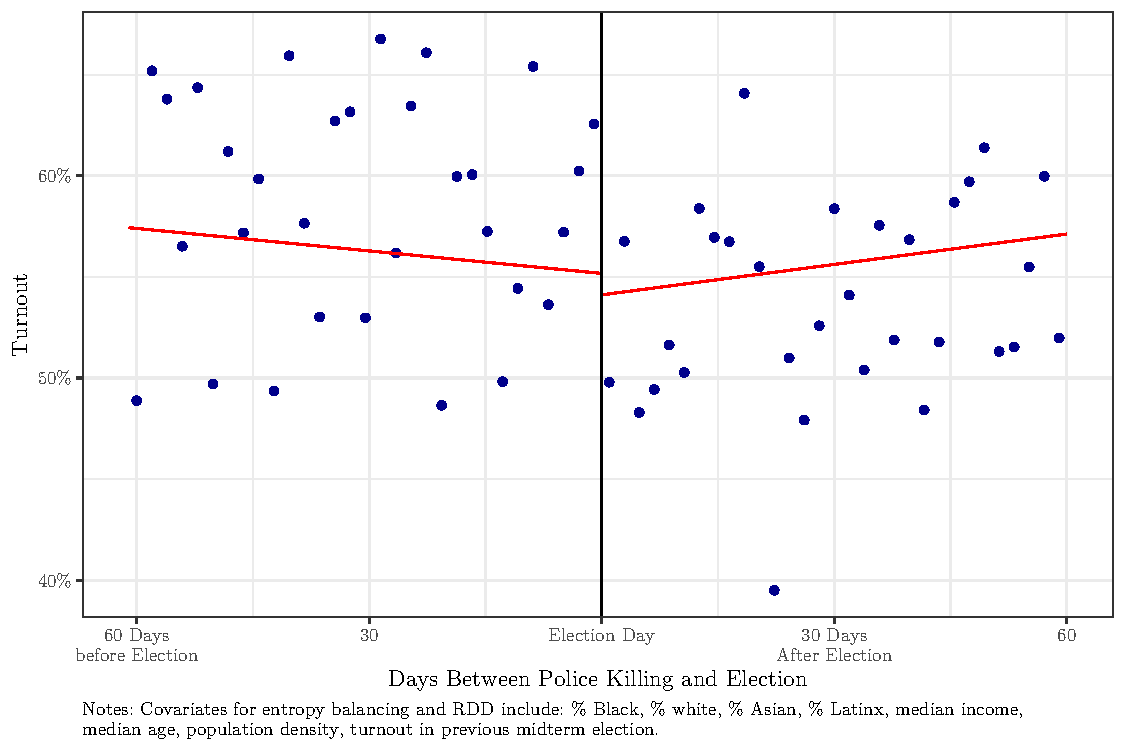
\includegraphics{shoot_to_files/figure-latex/rd2-chunk-1} 

}

\caption{\label{fig:map}RDD Plot, Covariates, 2016 and 2020}\label{fig:rd2-chunk}
\end{figure}

Now no processing at all---straight RD.

\begin{figure}[H]

{\centering 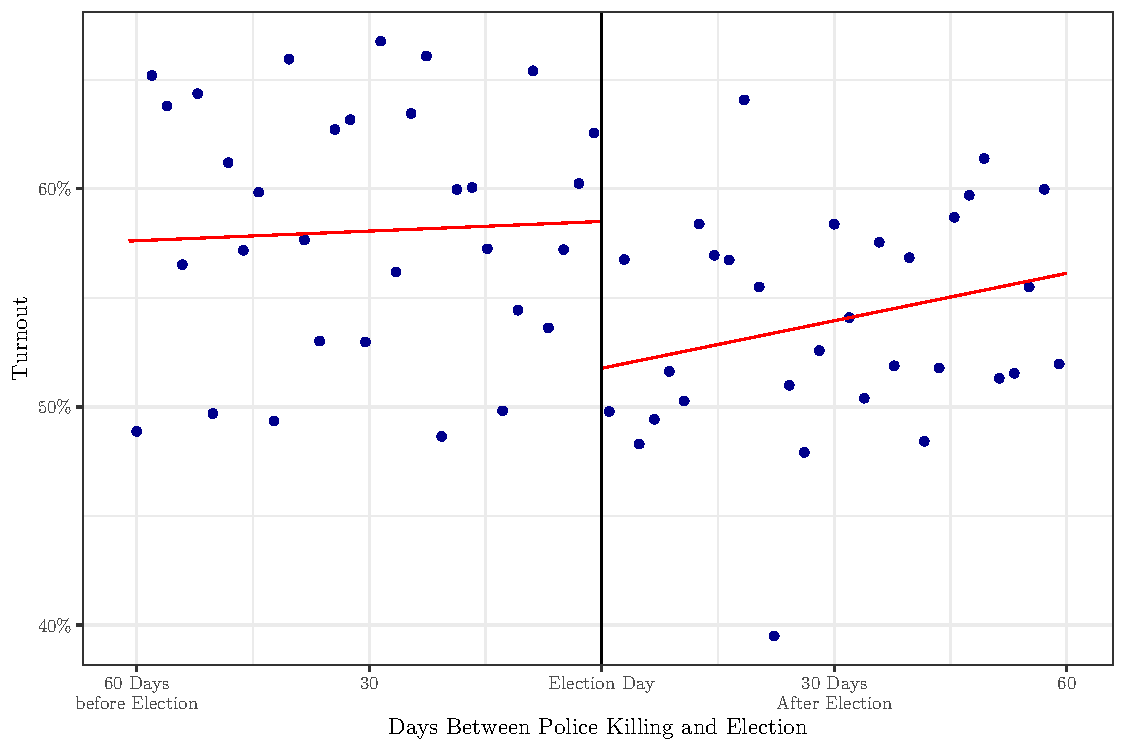
\includegraphics{shoot_to_files/figure-latex/rd3-chunk-1} 

}

\caption{\label{fig:map}RDD Plot, Unprocessed, 2016 and 2020}\label{fig:rd3-chunk}
\end{figure}

All these results also hold when the dependent variable is change in turnout from previous midterm election, rather than straight turnout.

There's also some conversation in the literature about what local polynomial should be around the cutpoint. We're robust to different polynomials (the charts above all use a polynomial of 1):

\begin{figure}[H]

{\centering 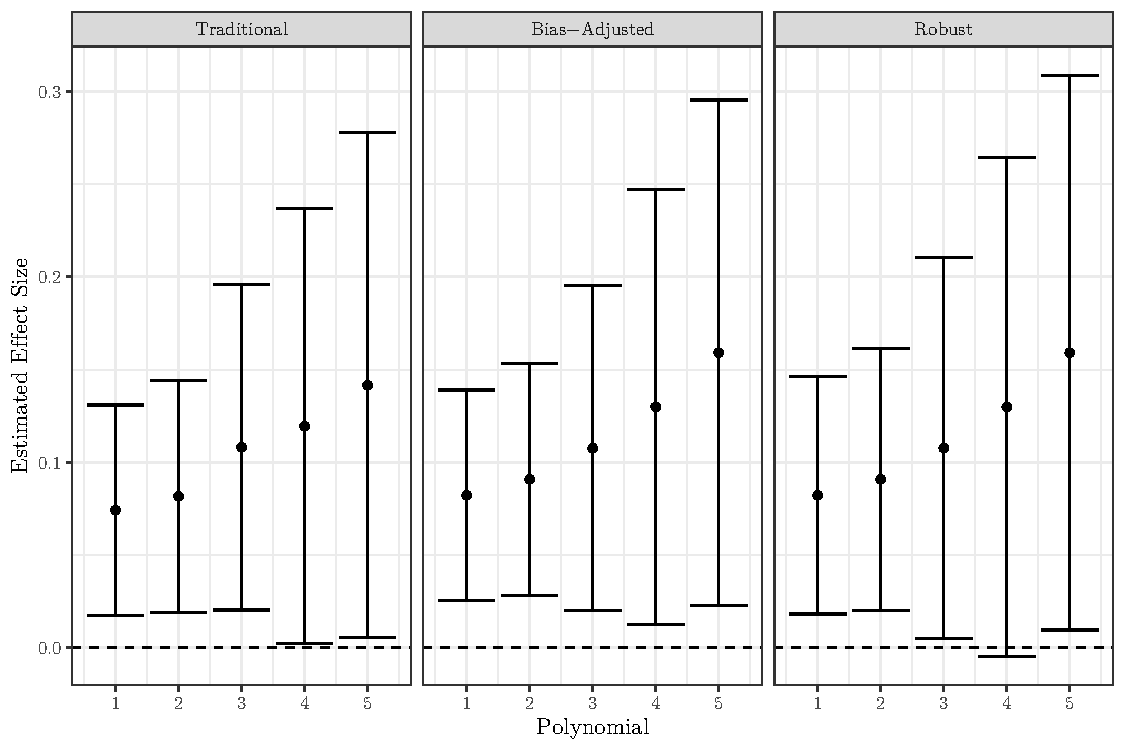
\includegraphics{shoot_to_files/figure-latex/polys-chunk-1} 

}

\caption{\label{fig:map}Estimated Effect Size, EB + Covariates, 2016 and 2020}\label{fig:polys-chunk}
\end{figure}

So that's everything with a 0.5 mile radius for turnout. Of course, we should see that any effect decays as we extend the distance between the killing and the killing. That's exactly what we do see:

\begin{figure}[H]

{\centering 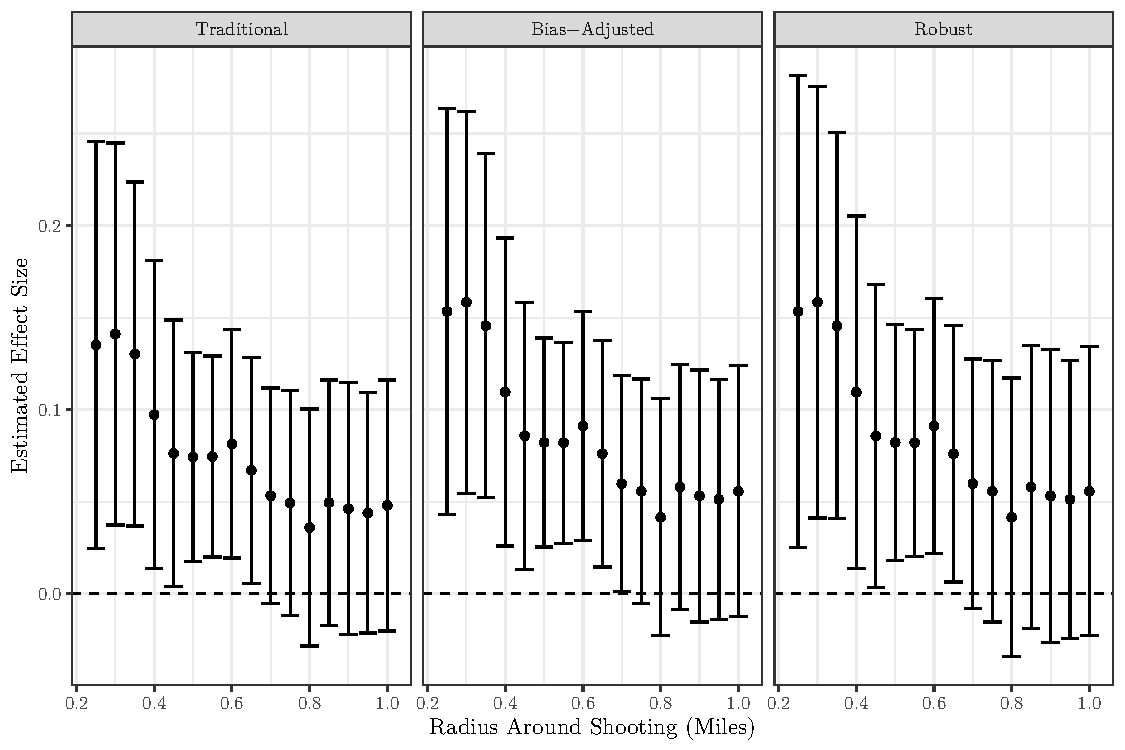
\includegraphics{shoot_to_files/figure-latex/dists-chunk-1} 

}

\caption{\label{fig:map}Estimated Effect Size, EB + Covariates, 2016 and 2020}\label{fig:dists-chunk}
\end{figure}

As we loosen the geographical proximity, we get smaller---and eventually nonsignificant---effects. These follow a nice trend, and are robust regardless of what standard errors / adjustment we use.

Somewhat surprisingly, these effects are driven largely by 2016. While the overall \emph{shape} is similar---very close block groups have a positive effect that decays---they never get nonsignificant in 2016.

Here's the 2016 plot:

\begin{figure}[H]

{\centering 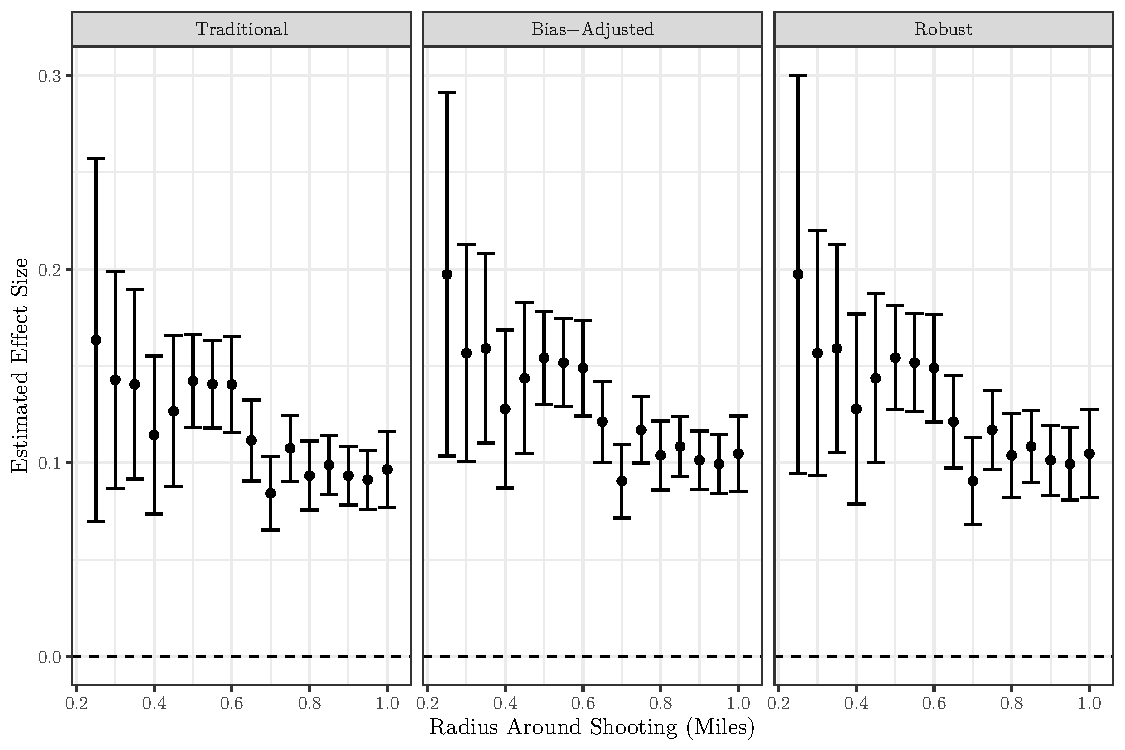
\includegraphics{shoot_to_files/figure-latex/dists-chunk16-1} 

}

\caption{\label{fig:map}Estimated Effect Size, EB + Covariates, 2016 Only}\label{fig:dists-chunk16}
\end{figure}

And for 2020:

\begin{figure}[H]

{\centering 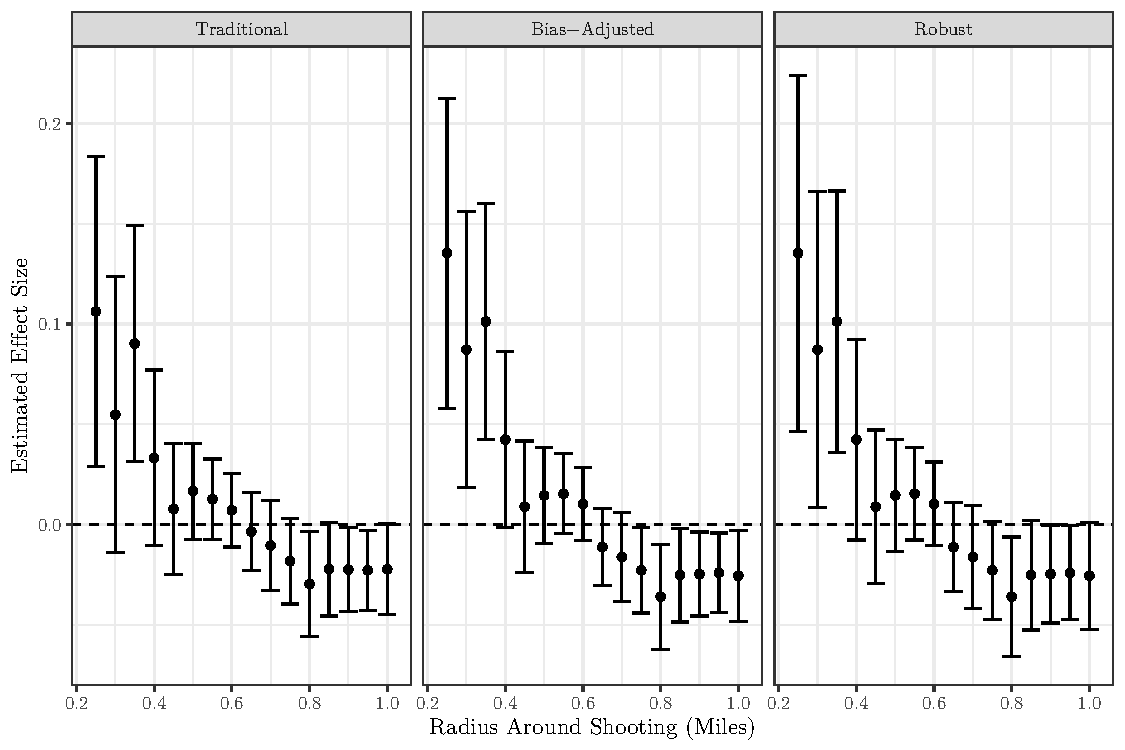
\includegraphics{shoot_to_files/figure-latex/dists-chunk20-1} 

}

\caption{\label{fig:map}Estimated Effect Size, EB + Covariates, 2020 Only}\label{fig:dists-chunk20}
\end{figure}

I haven't really looked to see if demos of the person killed / demos of the neighborhood moderate the treatment effect. Doing that is tricky in an RDD, and divvying up the observations into Black / non-Black neighborhoods, etc, starts to kill statistical power pretty quickly. So some more digging on that front needs to happen.

\hypertarget{vote-share}{%
\section*{Vote Share}\label{vote-share}}
\addcontentsline{toc}{section}{Vote Share}

Okay. So I'm reasonably convinced that there's a turnout effect. But the \textbf{major limitation} of the turnout effect alone is that we don't know what it means. Is this a rah-rah rally-around-the-flag, the-police-just-kept-me-safe, wohoo-government effect? Or is this evidence of voters holding the state accountable?

I'm not sure how to get at this question. I'd love to use timing in responses to the CCES to see if people who responded before / after a killing in their county had different views of the police, but the geographical effect goes away at a mile, so I don't know if I trust that. For now, I'm not sure if there's anything much stronger than Biden's vote share in each precinct.

So here's the estimated bump that Biden got in places with a killing immediately before the election:

\begin{figure}[H]

{\centering 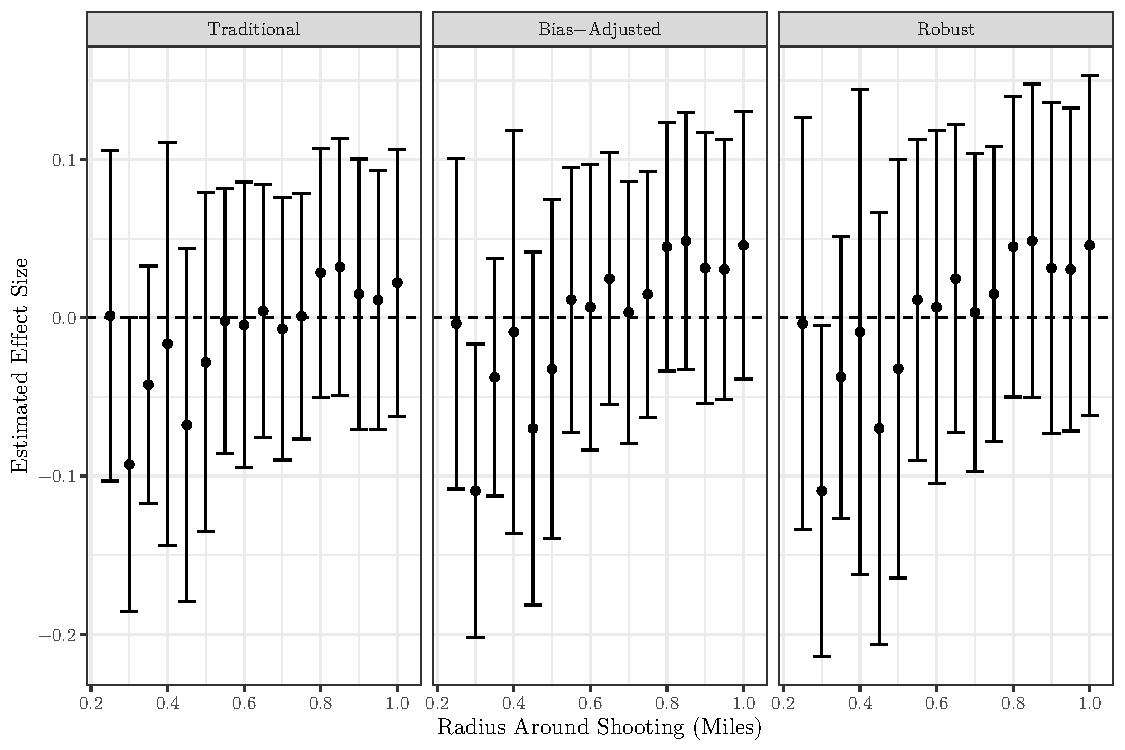
\includegraphics{shoot_to_files/figure-latex/dists-chunk-results-1} 

}

\caption{\label{fig:map}Estimated Effect Size, EB + Covariates, 2020 Only}\label{fig:dists-chunk-results}
\end{figure}

There's not much evidence of any effect here.

\newpage

\hypertarget{references}{%
\section*{References}\label{references}}
\addcontentsline{toc}{section}{References}

\hypertarget{refs}{}
\begin{CSLReferences}{1}{0}
\leavevmode\hypertarget{ref-Calonico2014}{}%
Calonico, Sebastian, Matias D. Cattaneo, and Rocio Titiunik. 2014. {``Robust {Nonparametric Confidence Intervals} for {Regression}-{Discontinuity Designs}.''} \emph{Econometrica} 82 (6): 2295--2326. \url{https://doi.org/10.3982/ECTA11757}.

\leavevmode\hypertarget{ref-Stommes2021}{}%
Stommes, Drew, P. M. Aronow, and Fredrik Sävje. 2021. {``On the Reliability of Published Findings Using the Regression Discontinuity Design in Political Science.''} September 29, 2021. \url{http://arxiv.org/abs/2109.14526}.

\end{CSLReferences}

\end{document}
